\chapter{Grundlagen}
\label{cha:Grundlagen}

\section{AMIDAR }
Bei der Klasse der AMIDAR Prozessoren handelt es sich um ein konfigurierbares System, bestehend aus Function Units (FU). Komplexe Instruktionen werden in mehrere Arbeitsschritte unterteilt, die als Token an die einzelnen FUs verteilt werden. Daf"ur wird das Token Distribution Network genutzt. F"ur die Kommunikation zwischen den FUs, gibt es auch noch einen Datenbus. Ein Vorteil der AMIDAR Architektur ist, dass leicht FUs eingef"ugt werden k"onnen, um den Prozessor an die Aufgaben anzupassen. Ein gutes Beispiel daf"ur sind die Hardwarebeschleuniger. \cite{Burkert}\cite{Andresen}

\begin{figure}[H]
	\centering
	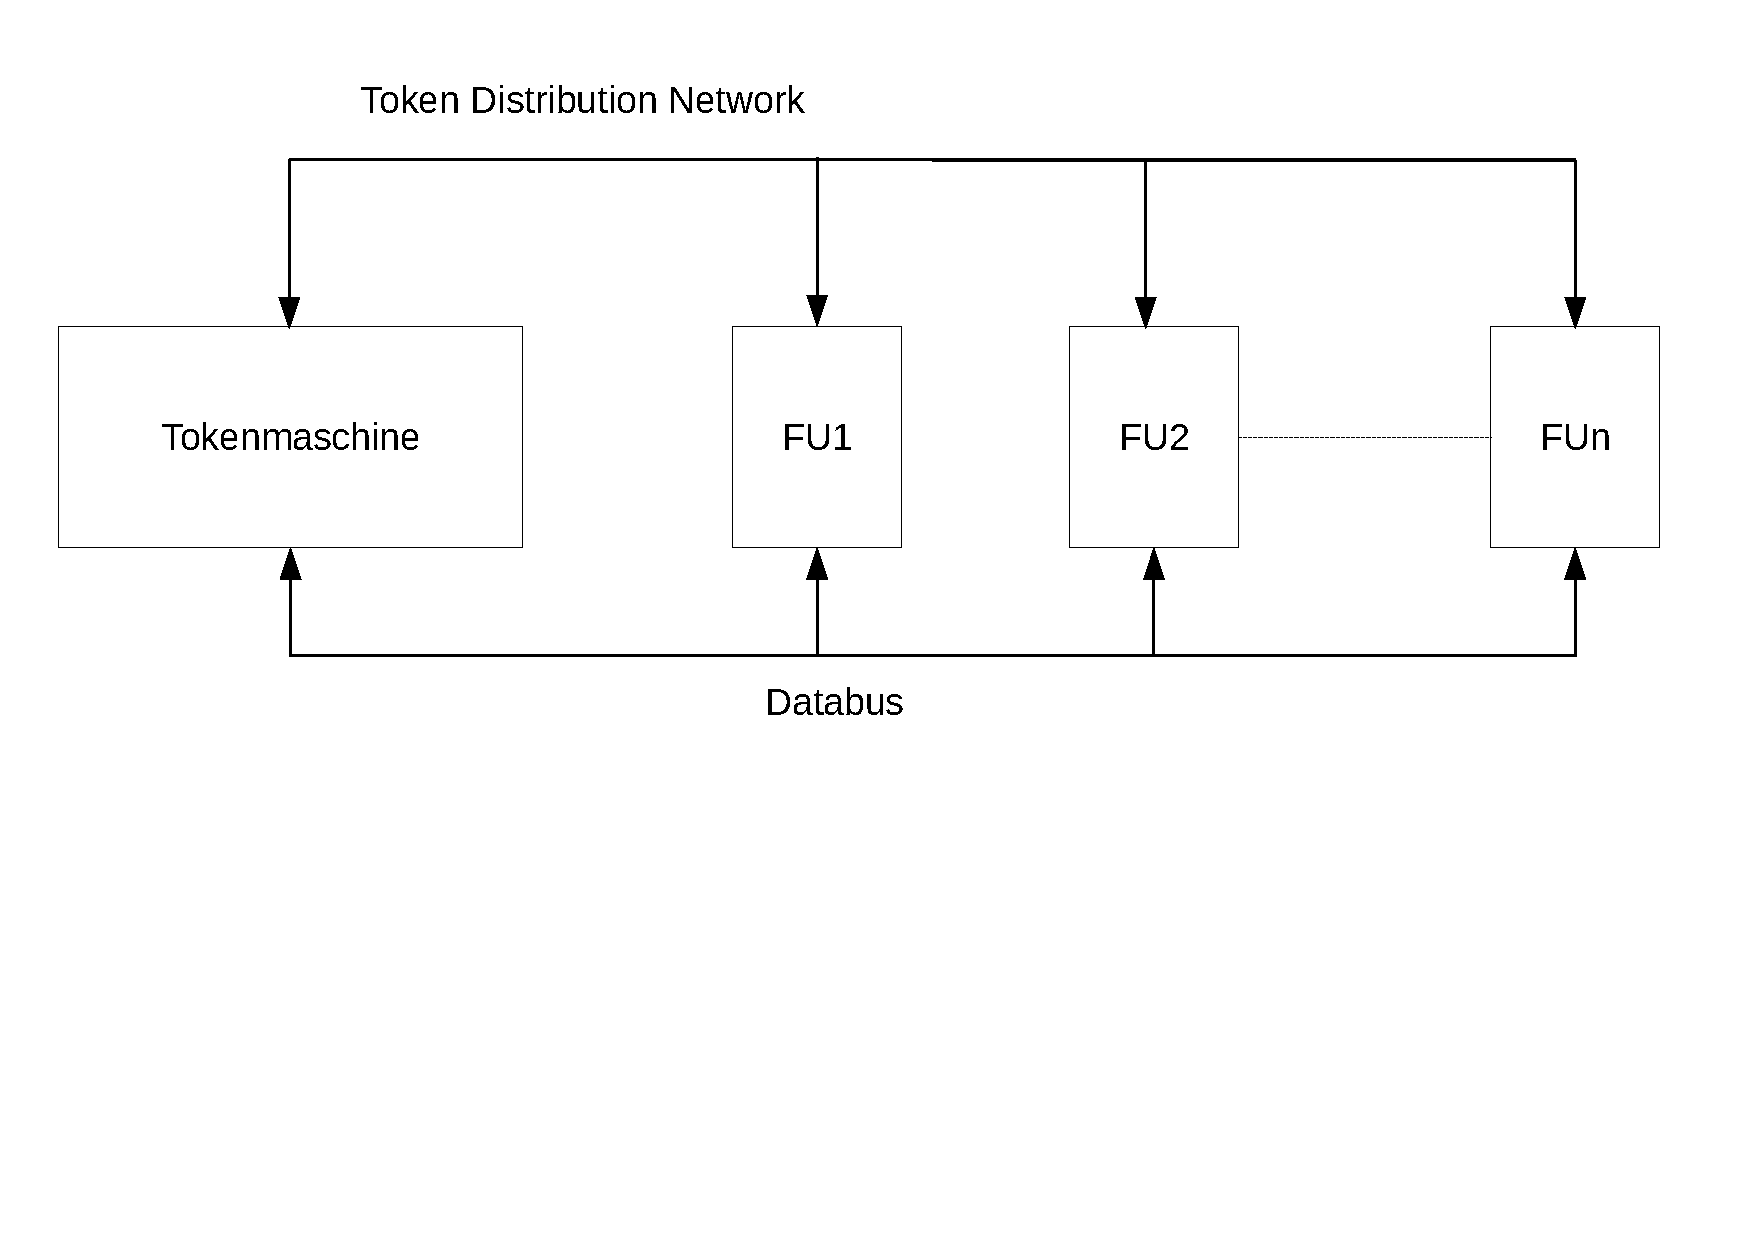
\includegraphics[height = 7cm]{PS_RS_graphics/AMIDAR.pdf}
	\caption{AMIDAR}
\end{figure}

\subsection{Lokale Variablen und Operanden in Java}
Java ist ein Objektorientierte Programmiersprache. Programme die in Java geschrieben worden sind, werden "ublicherweise in einer virtuellen Maschine ausgef"uhrt. 
Dabei werden Frames genutzt, die f"ur die Ausf"uhrung einer Methode wichtige Daten beinhalten. Ein Frame wird bei einen Methodenaufruf erzeugt und bei einen Methodenr"ucksprung zerst"ort. Ein Frame enh"alt jeweils den Speicher f"ur die lokalen Variablen, wie auch den Operandstack.  
Die Java Virtual Machine arbeitet Stackbasiert, was bedeutet, das Operanden nicht, wie in einer Registermaschine, in Registern gespeichert werden, sondern auf den Operandstack gelegt werden. Rechenoperationen und Funktionsaufrufe nehmen jeweils die obersten Werte des Operandstacks als Parameter. 

\subsection{Framestack}
Die AMIDAR Implementierung, die am Fachgebiet Rechnersysteme entwickelt wird, arbeitet mit Java Bytecode. Dabei wird der Stack f"ur Lokale Variablen und der Operandenstack in der Framestack FU zusammengefasst. Durch das Zusammenfassen beider Stacks, werden Kopiervorg"ange "uber den AMIDAR Bus eingespart. Zum einen m"ussten lokale Variablen bei jeder Verwendung auf den Operandstack kopiert werden, zum anderen m"ussten Parameter bei jeden Funktionsaufruf in den lokalen Variablenspeicher kopiert werden.
Der AMIDAR Framestack arbeitet bei der Stackframe Verarbeitung mit drei grunds"atzlichen Zeigern. Der Stackpointer gibt die n"achste freie Speicheradresse "uber den aktuellen Stackframe an. Der Locals Pointer gibt die unterste Lokale Variable und damit auch das untere Ende des Stackframes an. Der dritte wichtige Zeiger ist der Callercontext Pointer, der auf die unterste Adresse des Callercontext deutet. \cite{Illy}

\subsubsection{Stackframe}
Ein Stackframe beginnt mit den Parametern und den Lokalen Variablen.  Dar"uber kommt der Callercontext mit den alten Localspointer, Stackpointer und Callercontextpointer. Das obere Ende des Stackframes besteht aus dem Callercontext. 
\cite{Illy}

\subsubsection{Funktionsaufrufe}
\begin{figure}[H]
	\centering
	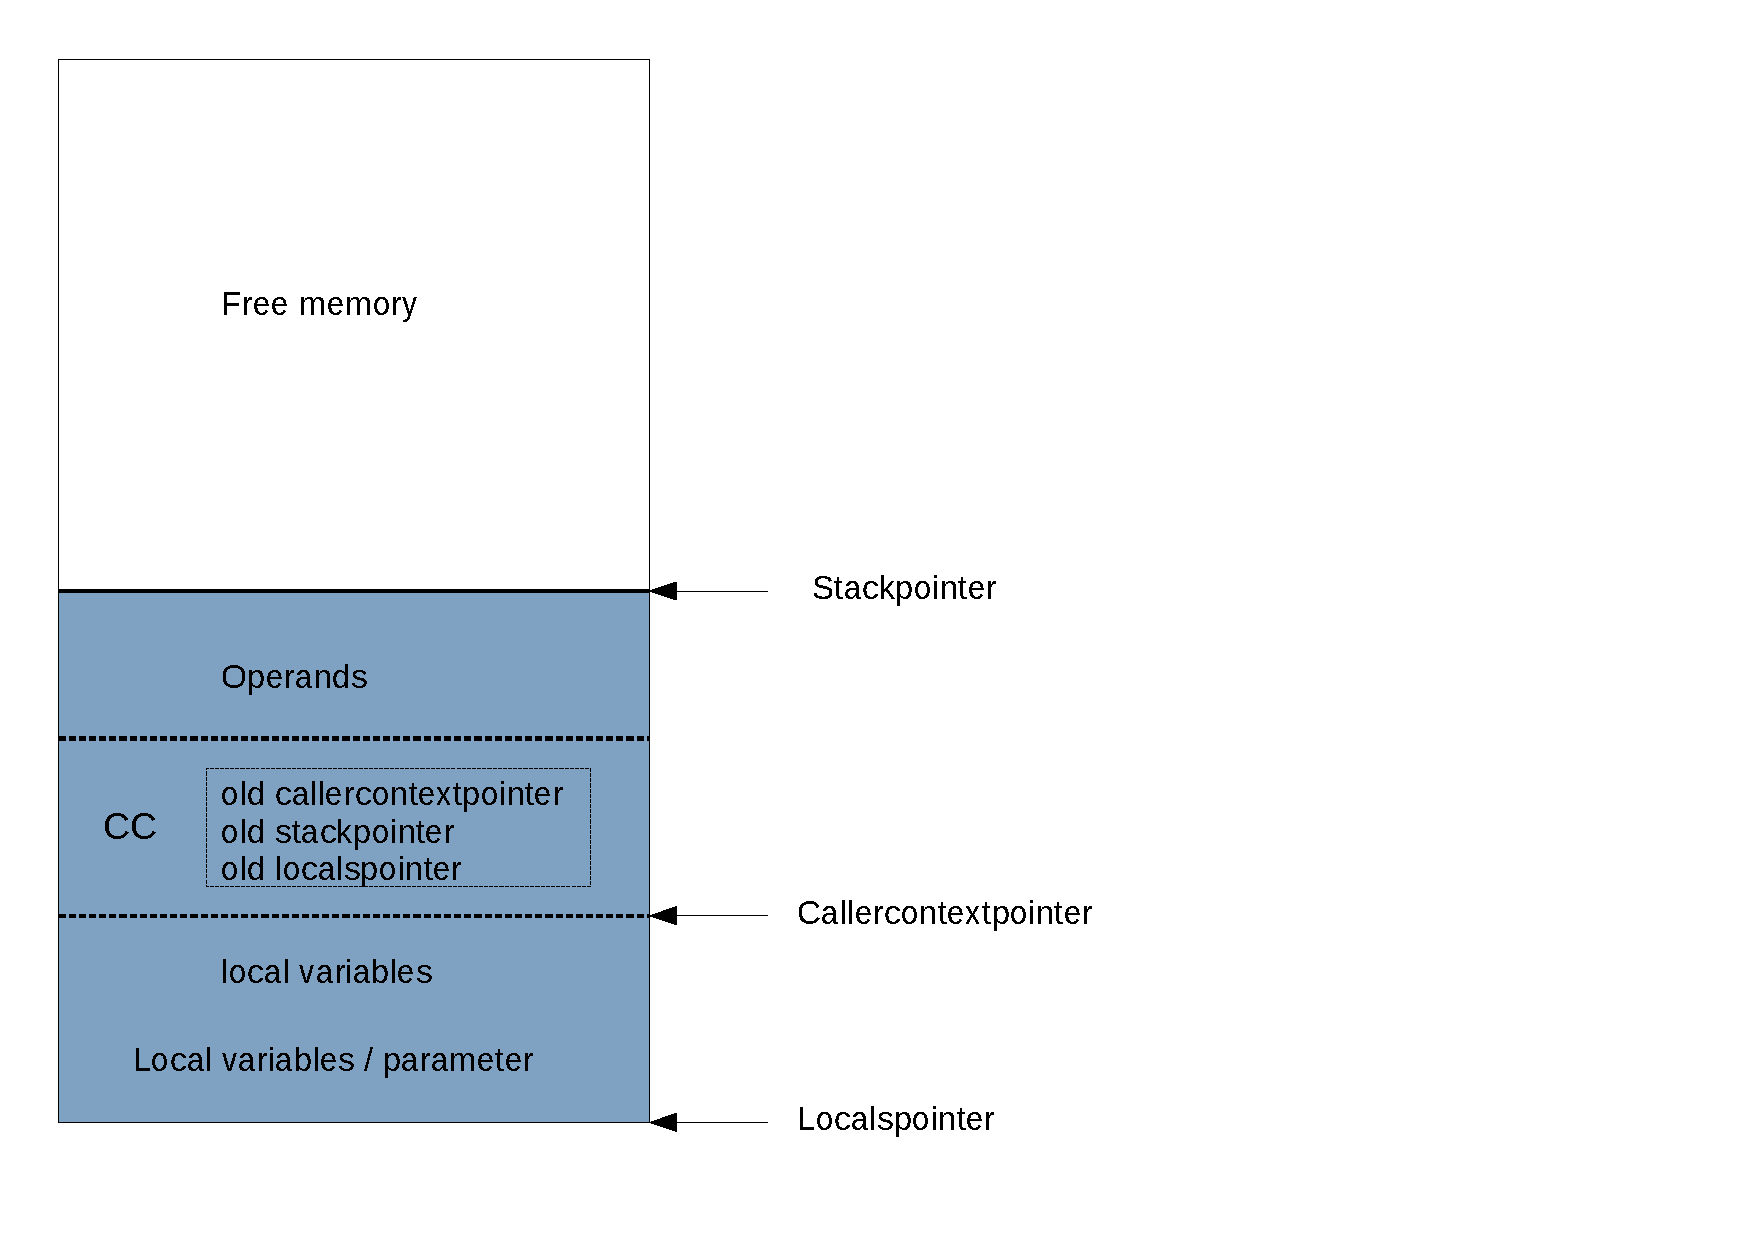
\includegraphics[height = 10cm]{PS_RS_graphics/StackframebeforeInvoke.pdf}
	\caption{Stackframe vor einen Funktionsaufruf}
\end{figure}
Eine f"ur dieses Projekt wichtige Funktion des Framestacks sind Funktionsaufrufe. Bei einen Funktionsaufruf werden im Framestack die 3 wichtigen Pointer neu gesetzt, wobei die alten Werte im Callercontext gesichert werden. Der neue Localspointer wird berechnet, in dem vom aktuellen Stackpointer die Anzahl der Parameter, der aufgerufenen Methode, abgezogen wird. Der neue Callercontextpointer wird berechnet, indem auf dem neuen Localspointer, die mit den Token "ubergebene, Anzahl lokaler Variablen addiert wird. Der neue Stackpointer wird berechnet, in dem auf dem Callercontextpointer die gr"o"ze des Callercontext addiert wird. 
In den n"achten Takten werden die alten Localspointer, Stackpointer und Callercontextpointer in den Callercontext geschrieben. \cite{Illy}
\begin{figure}[H]
	\centering
	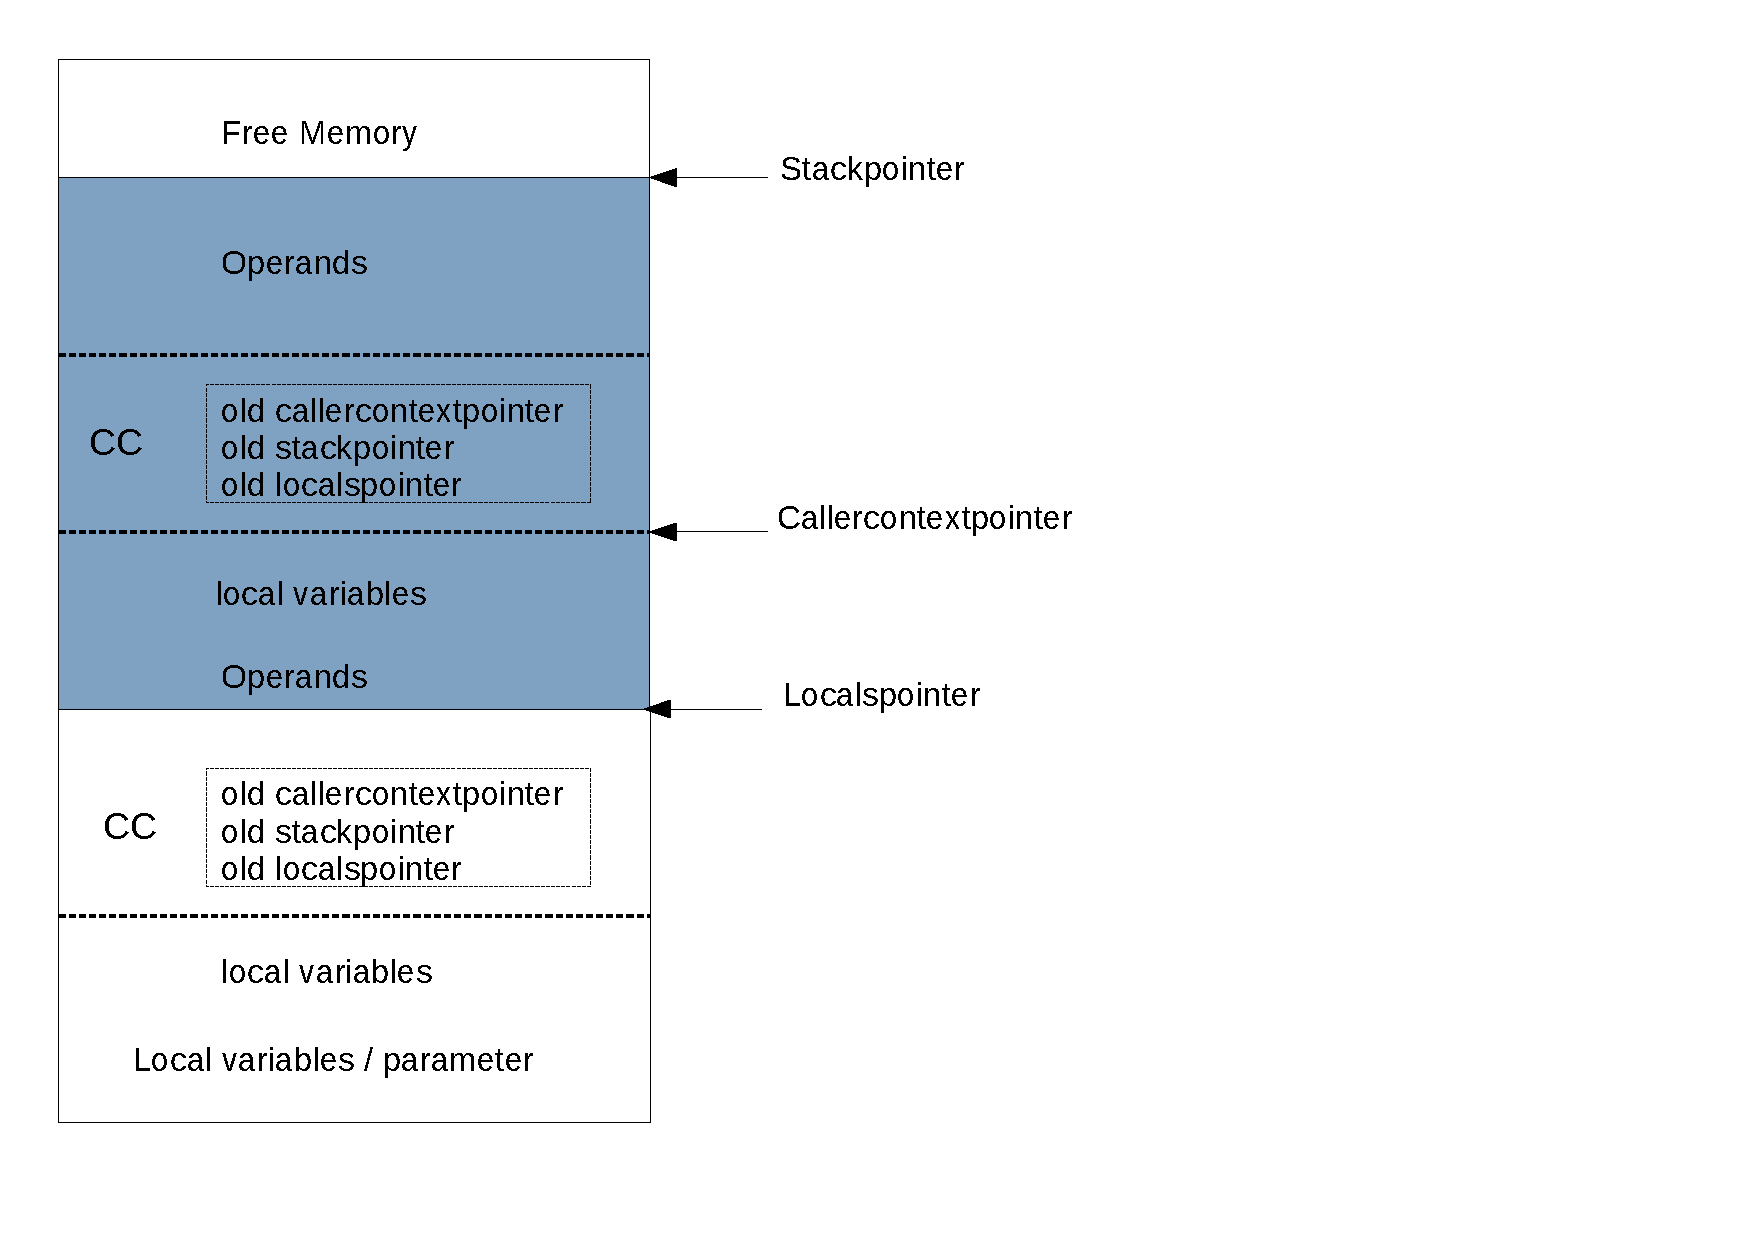
\includegraphics[height = 10cm]{PS_RS_graphics/StackframeafterInvoke.pdf}
	\caption{Stackframe nach einen Funktionsaufruf}
\end{figure}


\subsubsection{Funktionsr"ucksprung}

Bei einem Funktionsr"ucksprung werden im AMIDAR Framestack die Locals- Stack- und Callercontextpointer aktualisiert. Der Vorgang beginnt, wenn eines der entsprechenden Token "uber den AMDIAR Bus gesendet wird. Es gibt 3 Varianten des Tokens. Eine liefert keinen R"uckgabewert, die anderen geben jeweils 32 oder 64 Bit zur"uck. Wenn der Token abgearbeitet wird, werden nacheinander die drei Pointer ausgelesen und wiederhergestellt. Anschlie"zend wird gegebenenfalls der R"uckgabewerte gesichert, dieser steht in den top of Stack bzw. next of stack Registern. Der R"uckgabewert wird an Stelle des obersten, im Falle eines Return64 der oberen beiden, Operanden des Urspr"unglichen Funktionsaufruf gespeichert. \cite{Illy}

\begin{figure}[H]
	\centering
	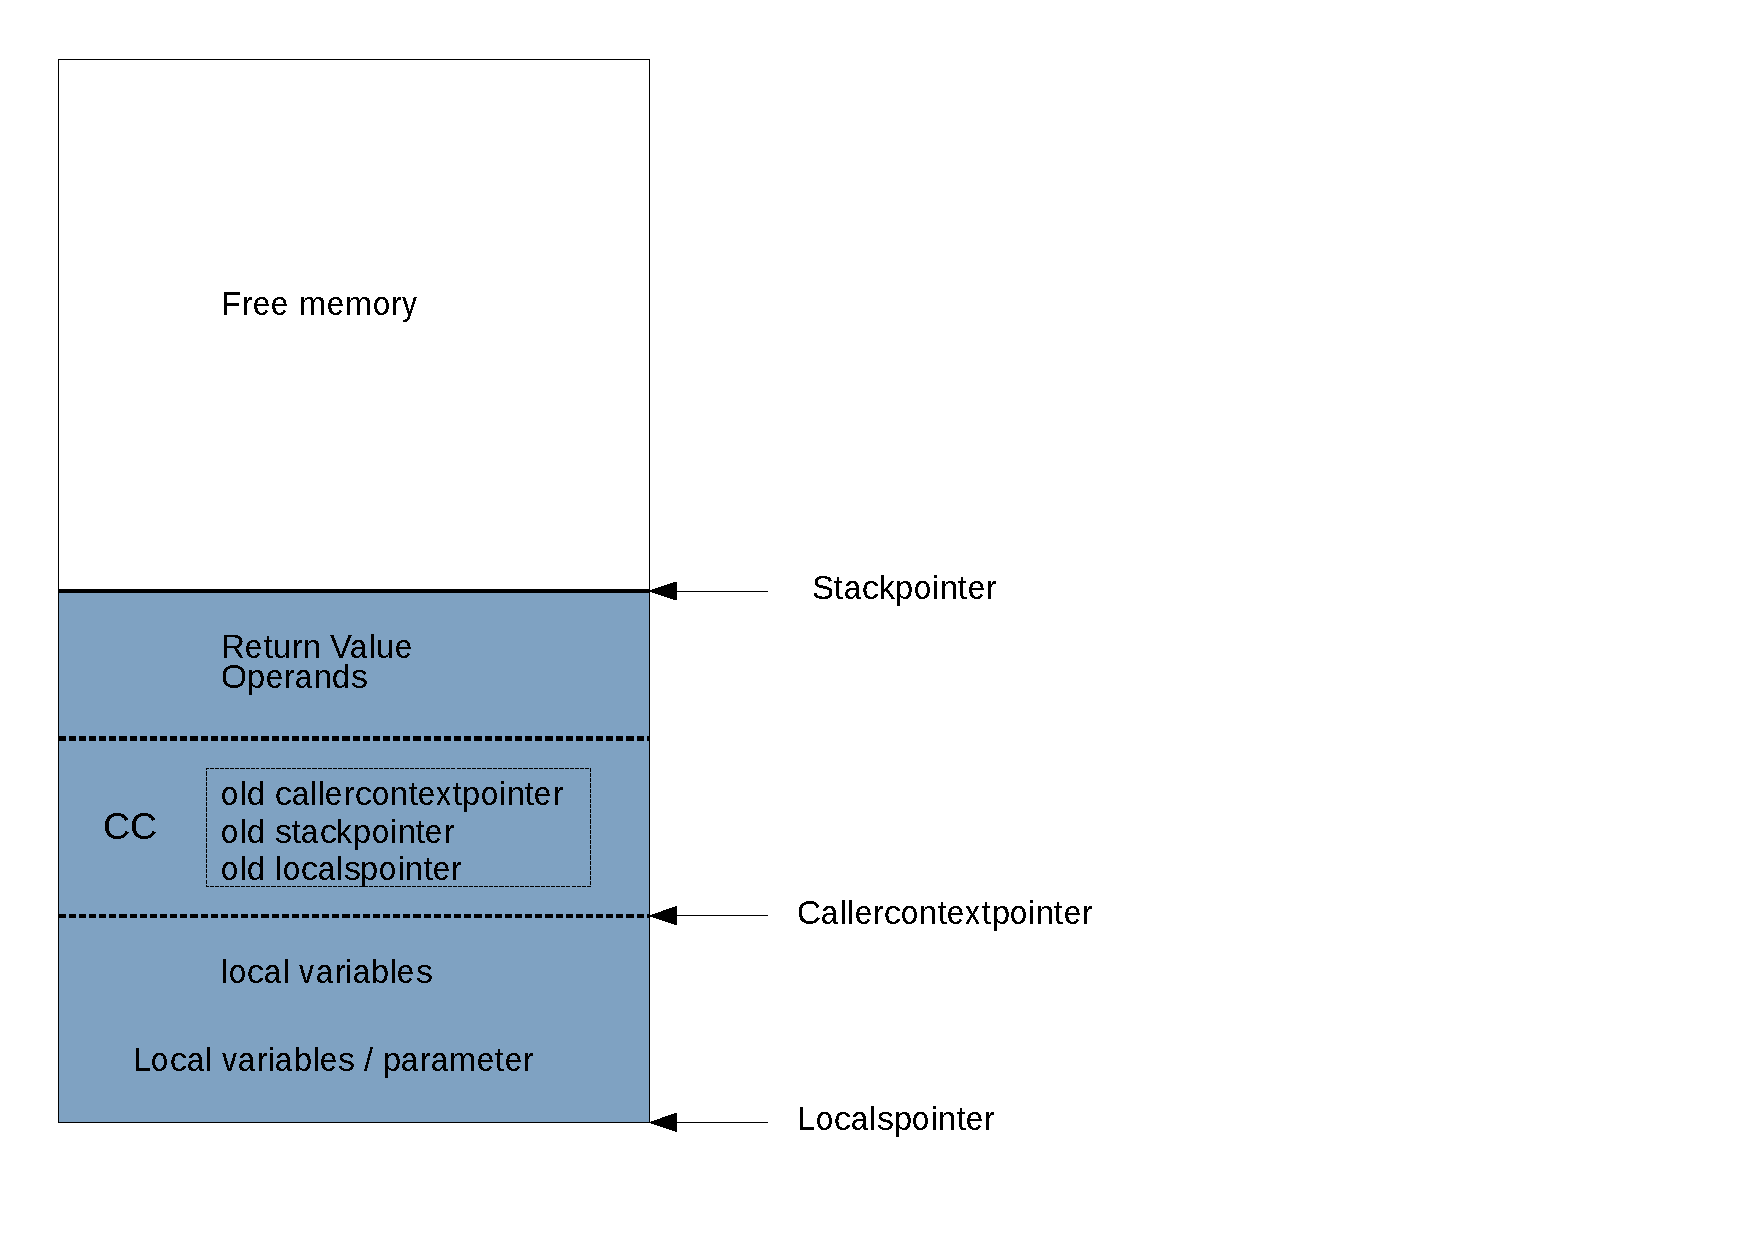
\includegraphics[height = 10cm]{PS_RS_graphics/Stackframeafterreturn.pdf}
	\caption{Stackframe nach einen Funktionsr"ucksprung}
\end{figure}
\section{Spill and Fill}

Spill and Fill beschreibt eine Strategie, durch die der Zugriff auf einen Stapelspeicher deutlich beschleunigt werden kann. Ein kleinerer, schnellerer Speicher h"alt einen Ausschnitt des Hauptspeichers vor, der je nach Bedarf hoch oder runter geschoben werden kann, sodass immer das obere Ende des Stapelspeichers im Window Ausschnitt liegt. Spill beschreibt dabei den Vorgang des nach oben Schiebens des Speicherausschnitts, bei den der untere Abschnitt des Ausschnitts in den Hauptspeicher geschrieben wird. Wird der Stack weit genug abgebaut, wird ein Fill durchgef"uhrt, bei dem die ausgelagerten Teile zur"uck kopiert werden.  

\begin{figure}[H]
	\centering
	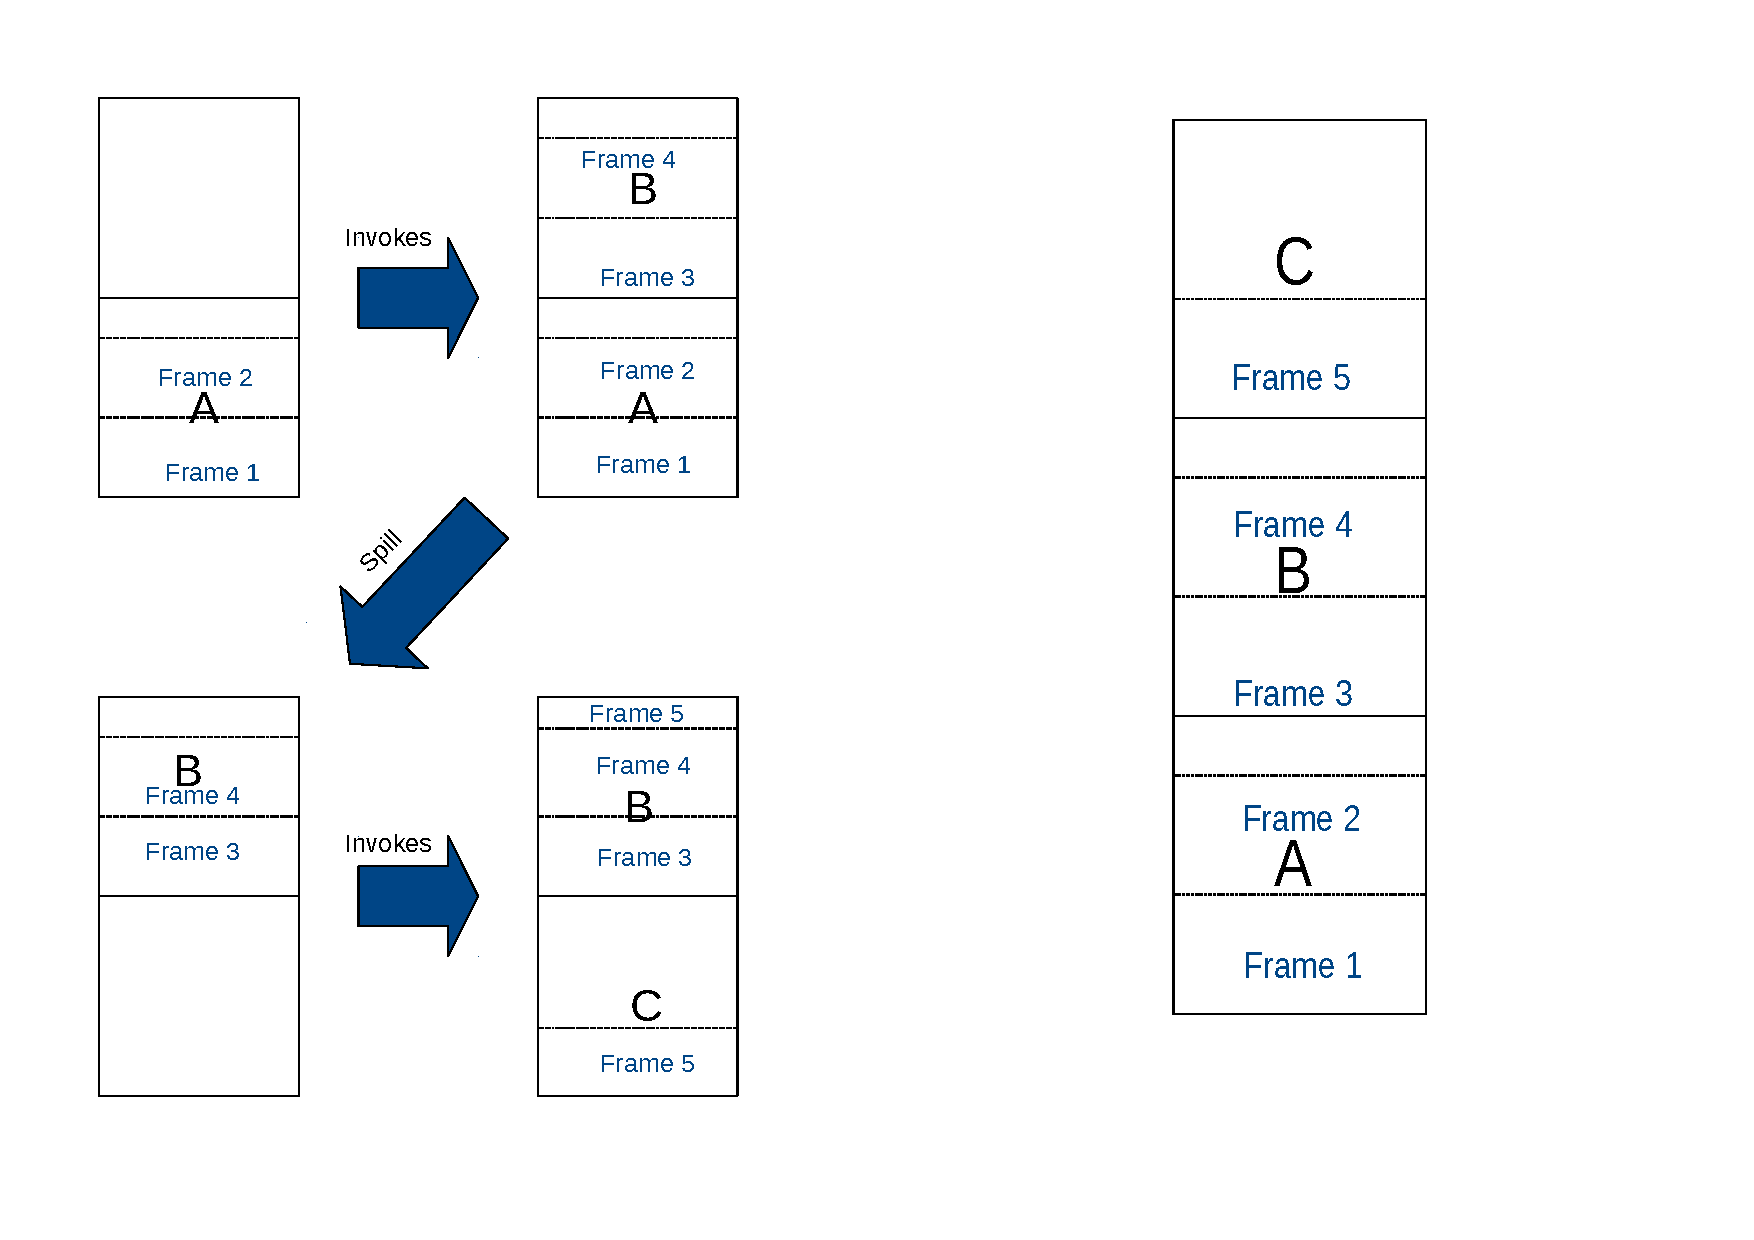
\includegraphics[height = 10cm]{PS_RS_graphics/spill.pdf}
	\caption{Spill: Verschieben des Windows }
\end{figure}

\begin{figure}[H]
	\centering
	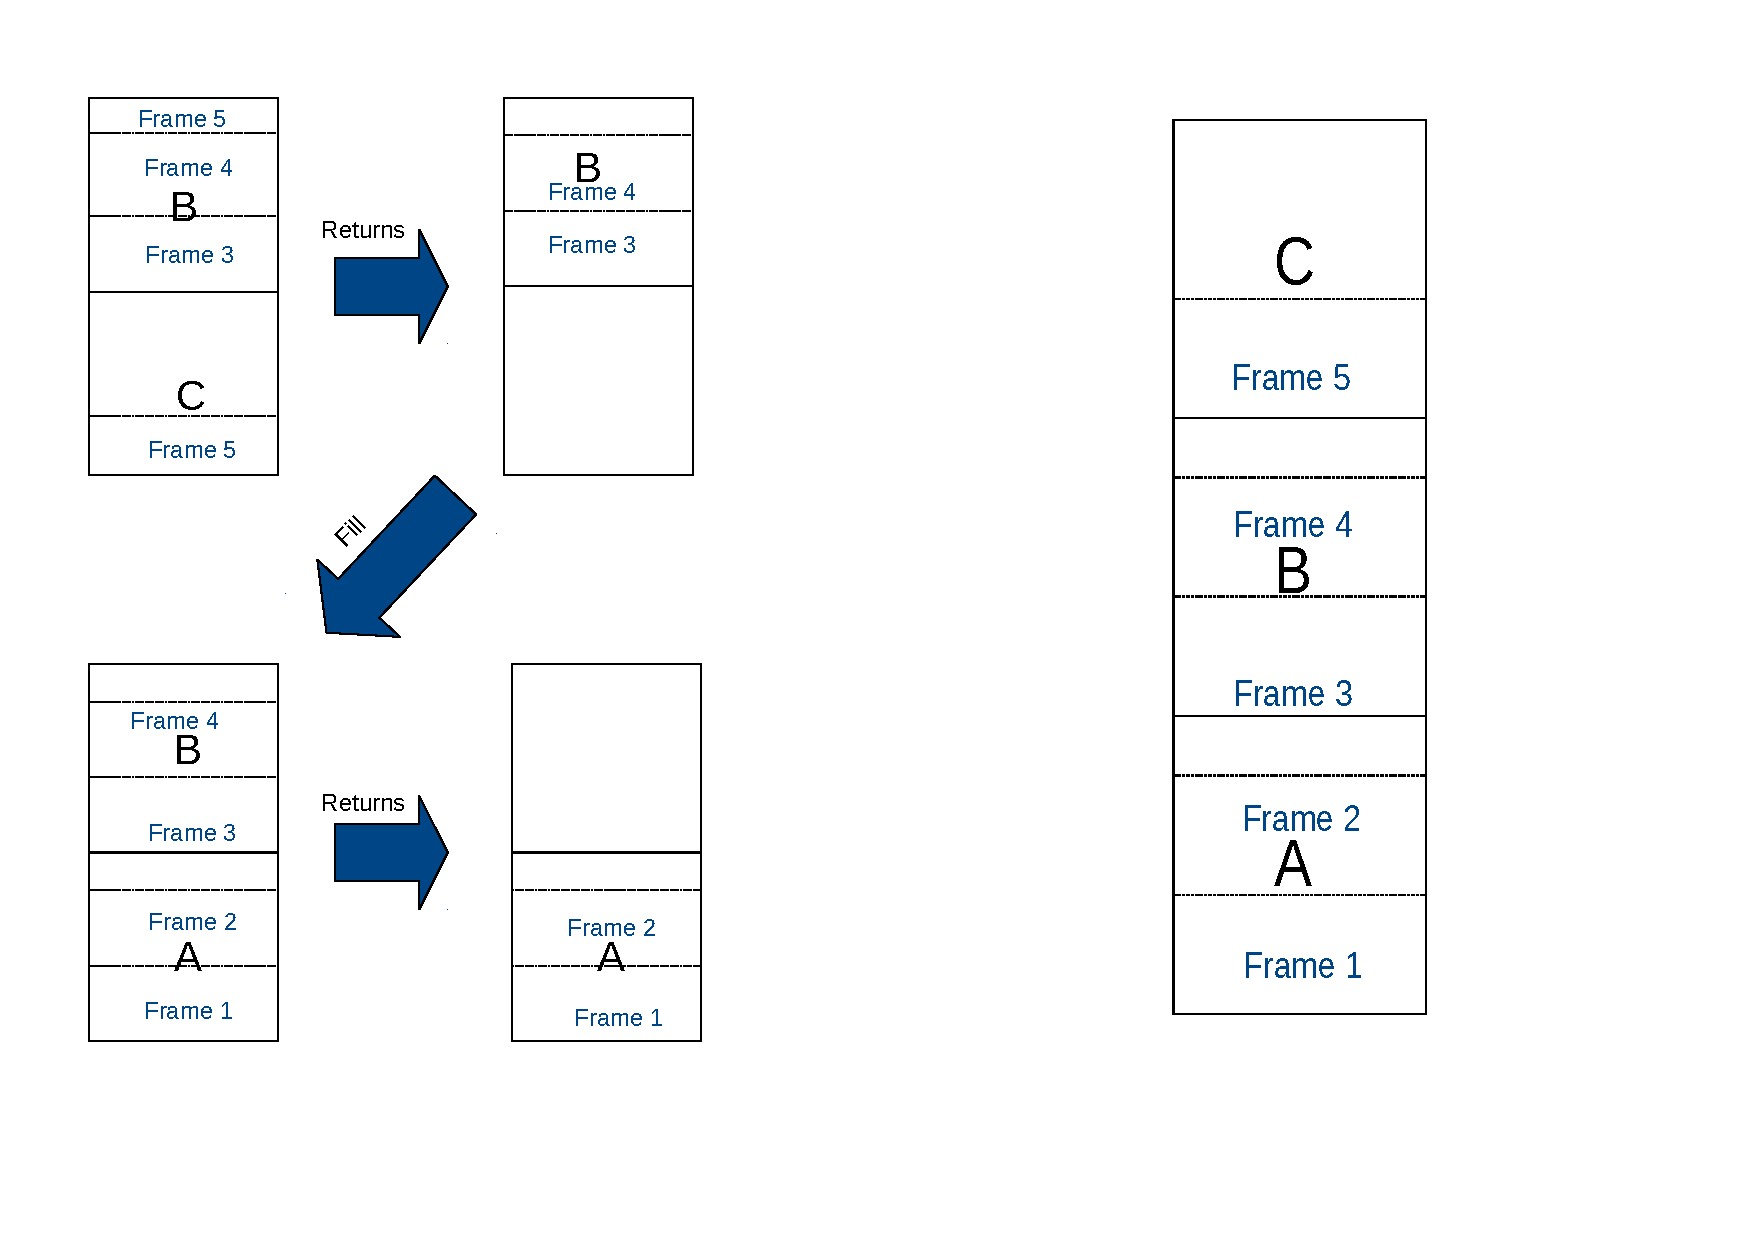
\includegraphics[height = 10cm]{PS_RS_graphics/fill.pdf}
	\caption{Fill: Verschieben des Windows}
\end{figure}


\begin{minipage}{\linewidth}
\section{Verwendung eines Spill and Fill Mechanismus in anderen Prozessoren}
\subsection{Sun Sparc Prozessoren}
Die Sun Sparc Prozessoren V8/V9 verf\"ugen \"uber ein sliding register Window mit jeweils 16 64 Bit gro"zen Registern in 7 Registers\"atzen. Sliding Window bezeichnet ein Verfahren, bei dem die Registers\"atze im Falle eines Funktionsaufruf nicht auf dem Stack gesichert werden m\"ussen, stattdessen wird auf den n\"achsten Registersatz gewechselt. Dabei wird meistens auch die Parameter\"ubergabe realisiert. Dabei sind die Input Register in dem Registerwindow des Callers identisch mit dem Output Registern, in dem Registerwindow des Callee.   
Mit speziellen Bytecode Instruktionen werden im Spill an Fill Verfahren Registers\"atze auf einen externen Speicher gesichert. Da das Spill and Fill durch spezielle Bytecodes ausgel"ost wird muss der Compiler vorher festlegen an welchen Stellen im Programm das Spill and Fill stattfinden soll. \cite{Gove}
\end{minipage}